\documentclass[theme=teal]{khmermath}

\geometry{left=0.85cm, right=0.85cm, top=0.75cm, bottom=1.5cm, footskip=0.7cm}
\usepackage{colortbl}
\usepackage{tikz}
\usetikzlibrary{calc,shapes,arrows,intersections,through,backgrounds,shadows,decorations.pathmorphing}

% Define arc accent
\newcommand{\wideparen}[1]{\overset{\boldsymbol{\frown}}{#1}}

% -------------------------------------------------------------------------
% Cohesive Color Palette: Teal Theme Template from example_exam.tex
% -------------------------------------------------------------------------
\definecolor{brandNavy}{RGB}{7, 94, 70}       % kmTealMain (Deep Emerald Teal)
\definecolor{brandBlue}{RGB}{0, 145, 155}     % kmTealSec (Ocean Cyan Teal)
\definecolor{brandLightBlue}{RGB}{244, 252, 250}% kmTealBg (Soft Mint Background)
\definecolor{brandCrimson}{RGB}{195, 35, 60}  % Crimson Red Accent
\definecolor{brandCoral}{RGB}{235, 80, 75}
\definecolor{brandGold}{RGB}{215, 130, 10}    % Warm Amber / Gold
\definecolor{brandGoldBg}{RGB}{255, 252, 242}
\definecolor{brandTeal}{RGB}{7, 94, 70}       % kmTealMain
\definecolor{brandTealBg}{RGB}{242, 252, 250}
\definecolor{subtleGray}{RGB}{246, 251, 249}
\definecolor{cardBorder}{RGB}{180, 225, 215}  % kmTealBorder

% Custom header & footer setup
\usepackage{fancyhdr}
\pagestyle{fancy}
\fancyhf{}
\renewcommand{\headrulewidth}{0pt}
\renewcommand{\footrule}{\color{brandNavy}\hrule height 0.8pt\vspace{3pt}}

\fancyfoot[L]{%
  \begin{tikzpicture}[baseline=(char.base)]
    \node[rounded corners=3.5pt, fill=brandNavy, text=white, font=\fontsize{8}{8}\selectfont\bfseries, inner sep=2.8pt] (char) {\ding{45}\ គណិតវិទ្យាសម្រាប់ថ្នាក់ទី៩};
  \end{tikzpicture}%
}
\fancyfoot[C]{%
  \fontsize{8.5}{8.5}\selectfont\kby \color{brandNavy}\textbf{\ding{72}\ បង្រៀនដោយ ៖ \textcolor{brandCrimson}{ក្រូត រស្មី}\ \ding{72}}%
}
\fancyfoot[R]{%
  
\begin{tikzpicture}[baseline=(char.base)]
    \node[rounded corners=3.5pt, fill=brandBlue!12, draw=brandBlue!40, line width=0.5pt, text=brandNavy, font=\fontsize{8}{8}\selectfont\bfseries, inner sep=2.5pt] (char) {\ding{37}\ Telegram: \textcolor{brandCrimson}{070897540}};
  \end{tikzpicture}%
}

% -------------------------------------------------------------------------
% Styled Boxes (tcolorbox)
% -------------------------------------------------------------------------
% General Rule Box (Teal/Emerald Theme - ជាទូទៅ)
\newtcolorbox{khboxorange}[1][]{
  enhanced,
  colframe=brandNavy!40,
  colback=brandLightBlue,
  boxrule=0.7pt,
  arc=5.0pt,
  borderline west={3.5pt}{0pt}{brandNavy},
  drop fuzzy shadow=brandNavy!15,
  left=10pt, right=10pt, top=7pt, bottom=6pt,
  title={\fontsize{9.5}{9.5}\selectfont\kml\color{white}\ding{72}\ ជាទូទៅ},
  coltitle=white,
  colbacktitle=brandNavy,
  boxed title style={
    boxrule=0pt,
    arc=3.5pt,
    left=7pt, right=7pt, top=2.5pt, bottom=2.5pt
  },
  attach boxed title to top left={yshift*=-\tcboxedtitleheight/2, xshift=12pt},
  #1
}

% General Rule Box (Teal/Emerald - ជាទូទៅ)
\newtcolorbox{khboxmagenta}[1][]{
  enhanced,
  colframe=brandNavy!40,
  colback=brandLightBlue,
  boxrule=0.7pt,
  arc=5.0pt,
  borderline west={3.5pt}{0pt}{brandNavy},
  drop fuzzy shadow=brandNavy!15,
  left=10pt, right=10pt, top=7pt, bottom=6pt,
  title={\fontsize{9.5}{9.5}\selectfont\kml\color{white}\ding{72}\ ជាទូទៅ},
  coltitle=white,
  colbacktitle=brandNavy,
  boxed title style={
    boxrule=0pt,
    arc=3.5pt,
    left=7pt, right=7pt, top=2.5pt, bottom=2.5pt
  },
  attach boxed title to top left={yshift*=-\tcboxedtitleheight/2, xshift=12pt},
  #1
}

% Practice Card Box
\newtcolorbox{khboxpractice}[1][]{
  enhanced,
  colframe=brandTeal,
  colback=brandTealBg,
  boxrule=0.9pt,
  arc=4pt,
  left=8pt, right=8pt, top=5pt, bottom=5pt,
  #1
}

% Example / Card Item Box
\newtcolorbox{khcard}[1][]{
  enhanced,
  colframe=cardBorder,
  colback=white,
  boxrule=0.7pt,
  arc=3.5pt,
  left=6pt, right=6pt, top=4pt, bottom=4pt,
  #1
}

% Section, Subsection & Header Badge Macros (Modern Pill Banners)
\newcommand{\khsection}[2]{%
  \vspace{6pt}%
  \noindent%
  \begin{tikzpicture}
    \fill[rounded corners=5pt, brandNavy!7] (0,0) rectangle (19.3, 0.72);
    \fill[rounded corners=4pt, brandNavy] (0.06, 0.06) rectangle (0.64, 0.66);
    \node[white, font=\fontsize{10}{10}\selectfont\bfseries] at (0.35, 0.36) {#1};
    \fill[brandGold, rounded corners=1pt] (0.74, 0.16) rectangle (0.78, 0.56);
    \node[anchor=west, font=\fontsize{11.5}{11.5}\selectfont\kml, color=brandCrimson] at (0.85, 0.36) {\textbf{#2}};
  \end{tikzpicture}%
  \vspace{3pt}%
}

\newcommand{\khsubsection}[2]{%
  \vspace{4pt}%
  \noindent%
  \begin{tikzpicture}[baseline=(sub.base)]
    \node[rounded corners=3.5pt, fill=brandBlue!12, draw=brandBlue!35, line width=0.5pt, text=brandNavy, font=\fontsize{9.5}{9.5}\selectfont\kml\bfseries, inner sep=3.5pt] (sub) at (0,0) {#1};
    \node[anchor=west, font=\fontsize{10.5}{10.5}\selectfont\kml\bfseries, color=brandNavy] at (sub.east) {\ \ #2};
  \end{tikzpicture}%
  \vspace{3pt}%
}

\newcommand{\secbadge}[1]{\tikz[baseline=(char.base)]{\node[circle, fill=brandNavy, inner sep=2.5pt, text=white, font=\fontsize{8.5}{8.5}\selectfont\bfseries] (char) {#1};}}
\newcommand{\alphabadge}[1]{\tikz[baseline=(char.base)]{\node[fill=brandCrimson, text=white, rounded corners=4pt, minimum size=15pt, inner sep=1pt, align=center, font=\fontsize{8.5}{8.5}\selectfont\bfseries] (char) {#1};}}

\newcommand{\exhead}[1]{\tikz[baseline=(char.base)]{\node[rounded corners=3.5pt, fill=brandCrimson!10, draw=brandCrimson!40, line width=0.5pt, text=brandCrimson, font=\fontsize{9.5}{9.5}\selectfont\kml\bfseries, inner sep=3pt] (char) {\small\ding{46}\ ឧទាហរណ៍#1};}}
\newcommand{\phead}{\tikz[baseline=(char.base)]{\node[rounded corners=3.5pt, fill=brandTeal!12, draw=brandTeal!45, line width=0.5pt, text=brandTeal!90!black, font=\fontsize{9.5}{9.5}\selectfont\kml\bfseries, inner sep=3pt] (char) {\small\ding{229}\ ប្រតិបត្តិ};}}
\newcommand{\exerhead}[1]{\tikz[baseline=(char.base)]{\node[rounded corners=3.5pt, fill=brandBlue!10, draw=brandBlue!40, line width=0.5pt, text=brandBlue, font=\fontsize{9.5}{9.5}\selectfont\kml\bfseries, inner sep=3pt] (char) {\small\ding{45}\ លំហាត់#1};}}
\newcommand{\samplehead}{\tikz[baseline=(char.base)]{\node[rounded corners=3.5pt, fill=brandCrimson!12, draw=brandCrimson!45, line width=0.5pt, text=brandCrimson, font=\fontsize{9.5}{9.5}\selectfont\kml\bfseries, inner sep=3pt] (char) {\small\ding{72}\ លំហាត់គំរូ};}}

\setlength{\parindent}{0pt}
\setlength{\parskip}{3.5pt}

\begin{document}

% =========================================================================
% PAGE 1: LESSON BANNER & SECTION 1.1
% =========================================================================
\noindent
\begin{tikzpicture}[x=1cm, y=1cm]
  \draw[rounded corners=6pt, fill=subtleGray, draw=gray!30, line width=0.5pt, drop shadow={shadow xshift=1pt, shadow yshift=-1pt, opacity=0.2}] 
    (0,0) rectangle (19.3, 2.35);

  % Top Color Accent Bar
  \fill[rounded corners=6pt, brandNavy] (0, 2.2) rectangle (19.3, 2.35);
  \fill[brandCrimson] (0, 2.2) rectangle (4.2, 2.35);
  \fill[brandGold] (4.2, 2.2) rectangle (6.8, 2.35);

  % Left Card: មេរៀនទី ១៣
  \draw[rounded corners=5pt, fill=white, draw=brandNavy!20, line width=0.8pt] 
    (0.3, 0.18) rectangle (3.8, 2.05);
  \node at (2.05, 1.6) {\fontsize{10}{10}\selectfont\kml\color{brandNavy} មេរៀនទី};
  \node at (2.05, 0.82) {\fontsize{23}{23}\selectfont\kml\color{brandCrimson} ១៣};

  % Center Card: ចំណងជើងមេរៀន រង្វង់និងបន្ទាត់
  \draw[rounded corners=5pt, fill=white, draw=brandBlue!25, line width=0.8pt] 
    (4.1, 0.18) rectangle (15.2, 2.05);
  \node at (9.65, 1.6) {\fontsize{11}{11}\selectfont\kml\color{brandBlue} ចំណងជើងមេរៀន};
  \node at (9.65, 0.82) {\fontsize{20}{20}\selectfont\kml\color{brandNavy} រង្វង់និងបន្ទាត់};
  \draw[brandGold, line width=0.9pt] (7.2, 0.4) -- (12.1, 0.4);
  \fill[brandGold] (9.65, 0.4) circle (2pt);

  % Right Card: ក្លឹបសិក្សា PCM
  \draw[rounded corners=5pt, fill=brandLightBlue, draw=brandBlue!30, line width=0.8pt] 
    (15.5, 0.18) rectangle (19.0, 2.05);
  \node at (17.25, 1.4) {\fontsize{9}{9}\selectfont\kml\color{brandNavy} ក្លឹបសិក្សាគណិតវិទ្យា};
  \node at (17.25, 0.72) {\fontsize{14}{14}\selectfont\bfseries\color{brandCrimson} PCM};
\end{tikzpicture}

\vspace{3pt}
\khsection{១}{លក្ខណៈនៃអង្កត់ធ្នូ}

\khsubsection{១.១}{បន្ទាត់កែងទៅនឹងចំណុចកណ្ដាលនៃអង្កត់ធ្នូ}

\begin{khboxorange}
  \begin{itemize}[leftmargin=15pt, itemsep=2pt, topsep=1pt, parsep=0pt]
    \item[\color{brandNavy}\ding{228}] \textbf{បន្ទាត់ដែលគូសចេញពីផ្ចិតនៃរង្វង់ហើយកែងនឹងអង្កត់ធ្នូត្រូវកាត់តាមចំណុចកណ្ដាលនៃអង្កត់ធ្នូ ។}
    \item[\color{brandNavy}\ding{228}] \textbf{បន្ទាត់ដែលកែងទៅនឹងចំណុចកណ្ដាលនៃអង្កត់ធ្នូត្រូវកាត់តាមផ្ចិតនៃរង្វង់ ។}
  \end{itemize}
\end{khboxorange}

\vspace{2pt}
\begin{khcard}
\begin{minipage}[c]{0.70\textwidth}
  ក្នុងរង្វង់ដូចរូបខាងស្ដាំ មានចំណុច $O$ ផ្ចិតនៃរង្វង់ $AB$ ជាអង្កត់ធ្នូ និង $OM$ ជាបន្ទាត់ដែលគូសកាត់ផ្ចិតរង្វង់ហើយកែងទៅនឹងអង្កត់ធ្នូ $AB$ ត្រង់ $M$ ។ គេទាញបាន ៖
  \begin{equation*}
    AM = BM = \frac{AB}{2}
  \end{equation*}
\end{minipage}\hfill
\begin{minipage}[c]{0.28\textwidth}
  \centering
  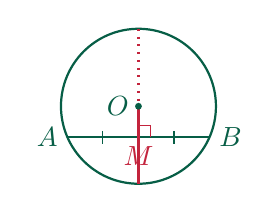
\begin{tikzpicture}[scale=0.82]
    \draw[thick, color=brandNavy] (0,0) circle (1.2);
    \coordinate (O) at (0,0);
    \coordinate (A) at (-1.1,-0.48);
    \coordinate (B) at (1.1,-0.48);
    \coordinate (M) at (0,-0.48);
    \draw[thick, color=brandNavy] (A) -- (B);
    \draw[thick, dotted, color=brandCrimson] (0,1.2) -- (0,0);
    \draw[thick, color=brandCrimson] (0,0) -- (0,-1.2);
    \fill[brandNavy] (O) circle (1.5pt) node[left] {$O$};
    \node[left, color=brandNavy] at (A) {$A$};
    \node[right, color=brandNavy] at (B) {$B$};
    \node[below, color=brandCrimson] at (M) {$M$};
    \draw[color=brandCrimson] (0,-0.3) -| (0.18,-0.48);
    \draw[color=brandNavy] (-0.55,-0.38) -- (-0.55,-0.58);
    \draw[color=brandNavy] (0.55,-0.38) -- (0.55,-0.58);
  \end{tikzpicture}
\end{minipage}
\end{khcard}

\vspace{2pt}
\begin{minipage}[c]{0.70\textwidth}
  \exhead{១} គេមានរង្វង់ផ្ចិត $O$ និងអង្កត់ធ្នូ $AB = 10\text{cm}$ ( ដូចរូប) ។\\
  បើ $OC$ កែងទៅនឹង $AB$ ចូរគណនាប្រវែង $AC$ ។
\end{minipage}\hfill
\begin{minipage}[c]{0.28\textwidth}
  \centering
  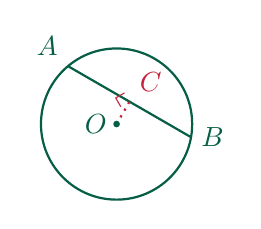
\begin{tikzpicture}[scale=0.80]
    \draw[thick, color=brandNavy] (0,0) circle (1.2);
    \coordinate (O) at (0,0);
    \coordinate (A) at (130:1.2);
    \coordinate (B) at (-10:1.2);
    \coordinate (C) at ($(A)!0.5!(B)$);
    \draw[thick, color=brandNavy] (A) node[above left] {$A$} -- (B) node[right] {$B$};
    \draw[thick, dotted, color=brandCrimson] (O) -- (C) node[above right, color=brandCrimson] {$C$};
    \fill[brandNavy] (O) circle (1.5pt) node[left] {$O$};
    \draw[rotate around={30:(C)}, color=brandCrimson] ($(C)+(0,0.16)$) -| ($(C)+(-0.16,0)$);
  \end{tikzpicture}
\end{minipage}

\vspace{2pt}
\begin{minipage}[c]{0.70\textwidth}
  \exhead{២} គេមានរង្វង់ផ្ចិត $O$ ( ដូចរូប) ។ ដែលមាន $OM = 5\text{cm}$\\
  និង $OB = 7\text{cm}$ ចូរគណនាប្រវែងអង្កត់ធ្នូ $AB$ ។
\end{minipage}\hfill
\begin{minipage}[c]{0.28\textwidth}
  \centering
  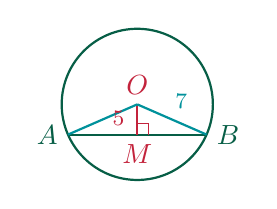
\begin{tikzpicture}[scale=0.80]
    \draw[thick, color=brandNavy] (0,0) circle (1.2);
    \coordinate (O) at (0,0);
    \coordinate (A) at (-1.1,-0.48);
    \coordinate (B) at (1.1,-0.48);
    \coordinate (M) at (0,-0.48);
    \draw[thick, color=brandNavy] (A) node[left] {$A$} -- (B) node[right] {$B$};
    \draw[thick, color=brandCrimson] (O) node[above] {$O$} -- (M) node[below] {$M$};
    \draw[thick, color=brandBlue] (O) -- (A);
    \draw[thick, color=brandBlue] (O) -- (B);
    \draw[color=brandCrimson] (0,-0.3) -| (0.18,-0.48);
    \node[left, color=brandCrimson] at (-0.05,-0.22) {\footnotesize $5$};
    \node[above right, color=brandBlue] at (0.45,-0.22) {\footnotesize $7$};
  \end{tikzpicture}
\end{minipage}

\vspace{2pt}
\begin{minipage}[c]{0.70\textwidth}
  \exhead{៣} នៅក្នុងរង្វង់ផ្ចិត $O$ គេមាន $\angle OXY = 30^\circ, \angle XOY = 60^\circ$\\
  និង $XZ = 32\text{cm}$ ចូរគណនារង្វាស់ $XY$ ។
\end{minipage}\hfill
\begin{minipage}[c]{0.28\textwidth}
  \centering
  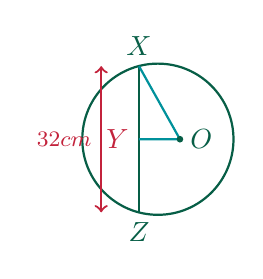
\begin{tikzpicture}[scale=0.80]
    \draw[thick, color=brandNavy] (0,0) circle (1.2);
    \coordinate (O) at (0.35,0);
    \coordinate (X) at (-0.3, 1.16);
    \coordinate (Z) at (-0.3, -1.16);
    \coordinate (Y) at (-0.3, 0);
    \draw[thick, color=brandNavy] (X) node[above] {$X$} -- (Z) node[below] {$Z$};
    \draw[thick, color=brandBlue] (X) -- (O) node[right, color=brandNavy] {$O$} -- (Y) node[left, color=brandCrimson] {$Y$};
    \fill[brandNavy] (O) circle (1.5pt);
    \draw[<->, thick, color=brandCrimson] (-0.9, 1.16) -- (-0.9, -1.16);
    \node[left, color=brandCrimson] at (-0.9, 0) {\footnotesize $32\text{cm}$};
  \end{tikzpicture}
\end{minipage}

\vspace{2pt}
\begin{khboxpractice}
\begin{minipage}[c]{0.70\textwidth}
  \phead\ គេមាន $O$ ជាផ្ចិតនៃរង្វង់ $AB = 25\text{cm}$ និង $BQ = 6.5\text{cm}$ ដូចរូបខាងស្ដាំនេះ ។ ចូរគណនាប្រវែង $AP$ និង $BC$ ។
\end{minipage}\hfill
\begin{minipage}[c]{0.28\textwidth}
  \centering
  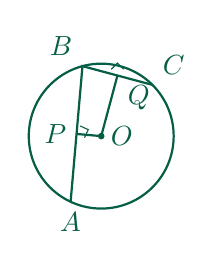
\begin{tikzpicture}[scale=0.80]
    \draw[thick, color=brandNavy] (0,0) circle (1.15);
    \coordinate (O) at (0,0);
    \coordinate (B) at (105:1.15);
    \coordinate (A) at (245:1.15);
    \coordinate (C) at (45:1.15);
    \coordinate (P) at ($(A)!0.5!(B)$);
    \coordinate (Q) at ($(B)!0.5!(C)$);
    \draw[thick, color=brandNavy] (A) node[below] {$A$} -- (B) node[above left] {$B$} -- (C) node[above right] {$C$};
    \draw[thick, color=brandTeal] (O) -- (P) node[left] {$P$};
    \draw[thick, color=brandTeal] (O) -- (Q) node[below right] {$Q$};
    \fill[brandNavy] (O) circle (1.5pt) node[right] {$O$};
    \draw[rotate around={-25:(P)}, color=brandTeal] ($(P)+(0.14,0)$) |- ($(P)+(0,0.14)$);
    \draw[rotate around={45:(Q)}, color=brandTeal] ($(Q)+(0.14,0)$) |- ($(Q)+(0,0.14)$);
  \end{tikzpicture}
\end{minipage}
\end{khboxpractice}

\vspace{6pt}
% -------------------------------------------------------------------------
% SECTION 1.2

\khsubsection{១.២}{អង្កត់ធ្នូស្មើគ្នា}

\begin{khboxorange}
  \begin{minipage}[c]{0.70\textwidth}
    \begin{itemize}[leftmargin=12pt, itemsep=3pt, topsep=1pt]
      \item[\color{brandNavy}\ding{228}] អង្កត់ធ្នូពីរមានប្រវែងស្មើគ្នានៅក្នុងរង្វង់មួយត្រូវមានចម្ងាយស្មើគ្នាពីផ្ចិតនៃរង្វង់នោះ ។
      \item[\color{brandNavy}\ding{228}] ច្រាសមកវិញ ៖ អង្កត់ធ្នូក្នុងរង្វង់មួយដែលមានចម្ងាយស្មើគ្នាពីផ្ចិតនៃរង្វង់ជាអង្កត់ធ្នូប៉ុនគ្នា ។
    \end{itemize}
  \end{minipage}\hfill
  \begin{minipage}[c]{0.26\textwidth}
    \centering
    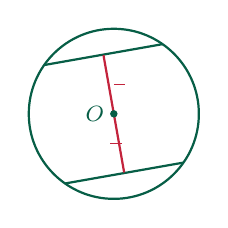
\begin{tikzpicture}[scale=0.90]
      \draw[thick, color=brandNavy] (0,0) circle (1.2);
      \coordinate (O) at (0,0);
      \draw[thick, color=brandNavy] (55:1.2) -- (145:1.2);
      \draw[thick, color=brandNavy] (-35:1.2) -- (-125:1.2);
      \draw[thick, color=brandCrimson] (O) -- (100:0.84);
      \draw[thick, color=brandCrimson] (O) -- (-80:0.84);
      \fill[brandNavy] (O) circle (1.5pt) node[left] {\footnotesize $O$};
      \draw[color=brandCrimson] (0, 0.42) -- (0.16, 0.42);
      \draw[color=brandCrimson] (-0.05, -0.42) -- (0.11, -0.42);
    \end{tikzpicture}
  \end{minipage}
\end{khboxorange}

\vspace{6pt}
\begin{khcard}
\begin{minipage}[c]{0.70\textwidth}
  \exhead{១} គេមានរង្វង់ផ្ចិត $O$ ដែលមានកាំ $5\text{cm}$ និងអង្កត់ធ្នូ $AB$ ប្រវែង $8\text{cm}$ ដូចរូបខាងស្ដាំ ។ ចូររកចម្ងាយពីផ្ចិតនៃរង្វង់ទៅអង្កត់ធ្នូ ។
\end{minipage}\hfill
\begin{minipage}[c]{0.28\textwidth}
  \centering
  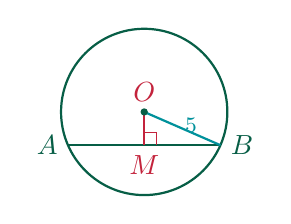
\begin{tikzpicture}[scale=0.88]
    \draw[thick, color=brandNavy] (0,0) circle (1.2);
    \coordinate (O) at (0,0);
    \coordinate (A) at (-1.1,-0.48);
    \coordinate (B) at (1.1,-0.48);
    \coordinate (M) at (0,-0.48);
    \draw[thick, color=brandNavy] (A) node[left] {$A$} -- (B) node[right] {$B$};
    \draw[thick, color=brandCrimson] (O) node[above] {$O$} -- (M) node[below] {$M$};
    \draw[thick, color=brandBlue] (O) -- (B);
    \fill[brandNavy] (O) circle (1.5pt);
    \draw[color=brandCrimson] (0,-0.3) -| (0.18,-0.48);
    \node[right, color=brandBlue] at (0.45,-0.2) {\footnotesize $5$};
  \end{tikzpicture}
\end{minipage}
\end{khcard}

\vspace{6pt}
\begin{khcard}
\begin{minipage}[c]{0.70\textwidth}
  \exhead{២} ក្នុងរូបខាងស្ដាំនេះ $O$ ជាផ្ចិតនៃរង្វង់ដែលមានកាំ $5\text{cm}$ ហើយ $PQ = RS = 6\text{cm}$ ។ ចូររកប្រវែង $OY$ និង $OX$ ។
\end{minipage}\hfill
\begin{minipage}[c]{0.28\textwidth}
  \centering
  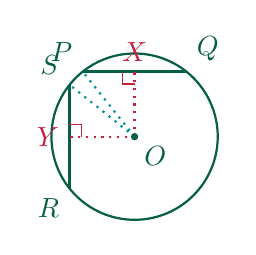
\begin{tikzpicture}[scale=0.88]
    \draw[thick, color=brandNavy] (0,0) circle (1.2);
    \coordinate (O) at (0,0);
    \coordinate (P) at (-0.75, 0.94);
    \coordinate (Q) at (0.75, 0.94);
    \coordinate (S) at (-0.94, 0.75);
    \coordinate (R) at (-0.94, -0.75);
    \draw[thick, color=brandNavy] (P) node[above left] {$P$} -- (Q) node[above right] {$Q$};
    \draw[thick, color=brandNavy] (S) node[above left] {$S$} -- (R) node[below left] {$R$};
    \draw[thick, dotted, color=brandCrimson] (O) -- (0, 0.94) node[above] {$X$};
    \draw[thick, dotted, color=brandCrimson] (O) -- (-0.94, 0) node[left] {$Y$};
    \draw[thick, dotted, color=brandBlue] (O) -- (P);
    \draw[thick, dotted, color=brandBlue] (O) -- (S);
    \fill[brandNavy] (O) circle (1.5pt) node[below right] {$O$};
    \draw[color=brandCrimson] (0, 0.76) -| (-0.18, 0.94);
    \draw[color=brandCrimson] (-0.76, 0) |- (-0.94, 0.18);
  \end{tikzpicture}
\end{minipage}
\end{khcard}

\vspace{6pt}
\begin{khcard}
\begin{minipage}[c]{0.70\textwidth}
  \exhead{៣} គេមានរង្វង់ផ្ចិត $O$ ដែលមានកាំ $10\text{cm}$ ហើយ $PR = QS$ និង $OC = 5\text{cm}$ ។ ចូរគណនាប្រវែង $OD$ និង $PR$ ។
\end{minipage}\hfill
\begin{minipage}[c]{0.28\textwidth}
  \centering
  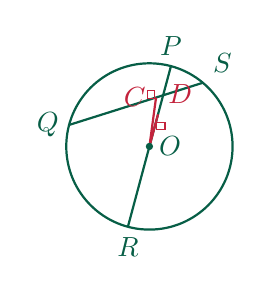
\begin{tikzpicture}[scale=0.88]
    \draw[thick, color=brandNavy] (0,0) circle (1.2);
    \coordinate (O) at (0,0);
    \coordinate (P) at (75:1.2);
    \coordinate (R) at (255:1.2);
    \coordinate (Q) at (165:1.2);
    \coordinate (S) at (50:1.2);
    \draw[thick, color=brandNavy] (P) node[above] {$P$} -- (R) node[below] {$R$};
    \draw[thick, color=brandNavy] (Q) node[left] {$Q$} -- (S) node[above right] {$S$};
    \coordinate (D) at ($(P)!0.3!(R)$);
    \coordinate (C) at ($(Q)!0.65!(S)$);
    \draw[thick, color=brandCrimson] (O) -- (D) node[above right] {$D$};
    \draw[thick, color=brandCrimson] (O) -- (C) node[left] {$C$};
    \fill[brandNavy] (O) circle (1.5pt) node[right] {$O$};
    \draw[color=brandCrimson] (D) ++(0.1, -0.12) rectangle ++(-0.12, -0.1);
    \draw[color=brandCrimson] (C) ++(-0.12, 0.1) rectangle ++(0.1, -0.12);
  \end{tikzpicture}
\end{minipage}
\end{khcard}

\vspace{6pt}
\begin{khboxpractice}
\begin{minipage}[c]{0.70\textwidth}
  \phead\ ក្នុងរូបខាងស្ដាំនេះគេមាន $O$ ជាផ្ចិតនៃរង្វង់ហើយ $OA = OB = 5.5\text{cm}$ និង $MN = 9\text{cm}$ ។ ចូររកប្រវែង $NP$ ។
\end{minipage}\hfill
\begin{minipage}[c]{0.28\textwidth}
  \centering
  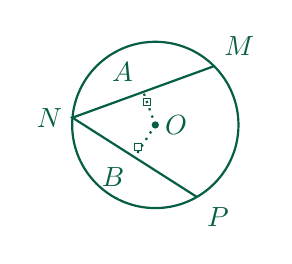
\begin{tikzpicture}[scale=0.88]
    \draw[thick, color=brandNavy] (0,0) circle (1.2);
    \coordinate (O) at (0,0);
    \coordinate (M) at (45:1.2);
    \coordinate (N) at (175:1.2);
    \coordinate (P) at (-60:1.2);
    \draw[thick, color=brandNavy] (M) node[above right] {$M$} -- (N) node[left] {$N$} -- (P) node[below right] {$P$};
    \coordinate (A) at ($(M)!0.5!(N)$);
    \coordinate (B) at ($(N)!0.5!(P)$);
    \draw[thick, dotted, color=brandTeal] (O) -- (A) node[above left] {$A$};
    \draw[thick, dotted, color=brandTeal] (O) -- (B) node[below left] {$B$};
    \fill[brandNavy] (O) circle (1.5pt) node[right] {$O$};
    \draw[color=brandTeal] (A) ++(0.1, -0.1) rectangle ++(-0.1, -0.1);
    \draw[color=brandTeal] (B) ++(0.1, 0.1) rectangle ++(-0.1, 0.1);
  \end{tikzpicture}
\end{minipage}
\end{khboxpractice}

\vspace{6pt}
% -------------------------------------------------------------------------
% SECTION 2 (TANGENTS)

\khsection{២}{បន្ទាត់ប៉ះ}

\begin{khboxmagenta}
  \begin{minipage}[c]{0.70\textwidth}
    \textbf{បន្ទាត់ប៉ះនៃរង្វង់ត្រូវកែងទៅនឹងកាំឬអង្កត់ផ្ចិតនៃរង្វង់ត្រង់ចំណុចប៉ះ ។}
  \end{minipage}\hfill
  \begin{minipage}[c]{0.26\textwidth}
    \centering
    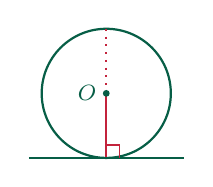
\begin{tikzpicture}[scale=0.82]
      \draw[thick, color=brandNavy] (0,0) circle (1.0);
      \coordinate (O) at (0,0);
      \draw[thick, dotted, color=brandCrimson] (0,1.0) -- (0,0);
      \draw[thick, color=brandCrimson] (0,0) -- (0,-1.0);
      \draw[thick, color=brandNavy] (-1.2,-1.0) -- (1.2,-1.0);
      \fill[brandNavy] (O) circle (1.5pt) node[left] {\footnotesize $O$};
      \draw[color=brandCrimson] (0,-0.8) -| (0.2,-1.0);
    \end{tikzpicture}
  \end{minipage}
\end{khboxmagenta}

\vspace{3pt}
\exhead{} តាមរូបនីមួយៗខាងក្រោម គេមានរង្វង់ផ្ចិត $O$ និង $PT$ ជាបន្ទាត់ប៉ះទៅនឹងរង្វង់ត្រង់ $T$

\vspace{5pt}
% 2x3 Grid of 6 Sub-Cases in elegant cards
\begin{minipage}[t]{0.32\textwidth}
  \begin{khcard}
    \centering
    \alphabadge{ក} ចូររកតម្លៃនៃមុំ $a$\\[4pt]
    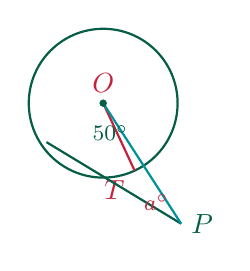
\begin{tikzpicture}[scale=0.90]
      \draw[thick, color=brandNavy] (0,0) circle (1.05);
      \coordinate (O) at (0,0);
      \coordinate (T) at (-65:1.05);
      \coordinate (P) at (1.1, -1.7);
      \draw[thick, color=brandCrimson] (O) node[above] {$O$} -- (T) node[below left] {$T$};
      \draw[thick, color=brandNavy] (-0.8, -0.55) -- (P) node[right] {$P$};
      \draw[thick, color=brandBlue] (O) -- (P);
      \node[color=brandNavy] at (0.1, -0.42) {\footnotesize $50^\circ$};
      \node[color=brandCrimson] at (0.75, -1.4) {\footnotesize $a^\circ$};
      \fill[brandNavy] (O) circle (1.5pt);
    \end{tikzpicture}
  \end{khcard}
\end{minipage}\hfill
\begin{minipage}[t]{0.32\textwidth}
  \begin{khcard}
    \centering
    \alphabadge{គ} ចូររកតម្លៃនៃមុំ $b$\\[4pt]
    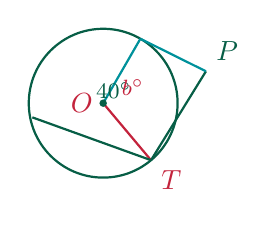
\begin{tikzpicture}[scale=0.90]
      \draw[thick, color=brandNavy] (0,0) circle (1.05);
      \coordinate (O) at (0,0);
      \coordinate (T) at (-50:1.05);
      \coordinate (P) at (1.45, 0.45);
      \coordinate (X) at (60:1.05);
      \draw[thick, color=brandCrimson] (O) node[left] {$O$} -- (T) node[below right] {$T$};
      \draw[thick, color=brandBlue] (O) -- (X);
      \draw[thick, color=brandNavy] (T) -- (P) node[above right] {$P$};
      \draw[thick, color=brandBlue] (X) -- (P);
      \draw[thick, color=brandNavy] (-1.0, -0.2) -- (T);
      \node[color=brandNavy] at (0.15, 0.18) {\footnotesize $40^\circ$};
      \node[color=brandCrimson] at (0.42, 0.22) {\footnotesize $b^\circ$};
      \fill[brandNavy] (O) circle (1.5pt);
    \end{tikzpicture}
  \end{khcard}
\end{minipage}\hfill
\begin{minipage}[t]{0.32\textwidth}
  \begin{khcard}
    \centering
    \alphabadge{ង} រកតម្លៃនៃមុំ $a, b$ និង $c$\\[4pt]
    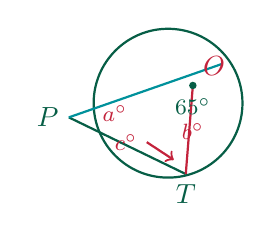
\begin{tikzpicture}[scale=0.90]
      \draw[thick, color=brandNavy] (0,0) circle (1.05);
      \coordinate (O) at (0.35, 0.25);
      \coordinate (T) at (0.25, -1.0);
      \coordinate (P) at (-1.4, -0.2);
      \draw[thick, color=brandNavy] (P) node[left] {$P$} -- (T) node[below] {$T$};
      \draw[thick, color=brandBlue] (P) -- (0.75, 0.55);
      \draw[thick, color=brandCrimson] (O) node[above right] {$O$} -- (T);
      \node[color=brandCrimson] at (-0.75, -0.15) {\footnotesize $a^\circ$};
      \node[color=brandNavy] at (0.35, -0.05) {\footnotesize $65^\circ$};
      \node[color=brandCrimson] at (0.35, -0.4) {\footnotesize $b^\circ$};
      \draw[->, color=brandCrimson, thick] (-0.3, -0.55) -- (0.08, -0.8);
      \node[left, color=brandCrimson] at (-0.3, -0.55) {\footnotesize $c^\circ$};
      \fill[brandNavy] (O) circle (1.5pt);
    \end{tikzpicture}
  \end{khcard}
\end{minipage}

\vspace{6pt}
\begin{minipage}[t]{0.32\textwidth}
  \begin{khcard}
    \centering
    \alphabadge{ខ} ចូររកតម្លៃនៃមុំ $a$ និង $b$\\[4pt]
    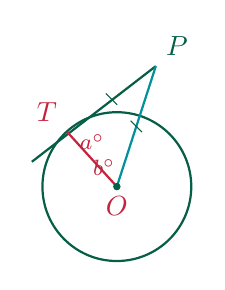
\begin{tikzpicture}[scale=0.90]
      \draw[thick, color=brandNavy] (0, -0.35) circle (1.05);
      \coordinate (O) at (0, -0.35);
      \coordinate (T) at (-0.7, 0.42);
      \coordinate (P) at (0.55, 1.35);
      \draw[thick, color=brandNavy] (-1.2, 0.0) -- (P) node[above right] {$P$};
      \draw[thick, color=brandCrimson] (O) node[below] {$O$} -- (T) node[above left] {$T$};
      \draw[thick, color=brandBlue] (O) -- (P);
      \draw[color=brandNavy] ($(T)!0.5!(P)+(-0.08,0.08)$) -- ($(T)!0.5!(P)+(0.08,-0.08)$);
      \draw[color=brandNavy] ($(O)!0.5!(P)+(-0.08,0.08)$) -- ($(O)!0.5!(P)+(0.08,-0.08)$);
      \node[color=brandCrimson] at (-0.35, 0.28) {\footnotesize $a^\circ$};
      \node[color=brandCrimson] at (-0.18, -0.08) {\footnotesize $b^\circ$};
      \fill[brandNavy] (O) circle (1.5pt);
    \end{tikzpicture}
  \end{khcard}
\end{minipage}\hfill
\begin{minipage}[t]{0.32\textwidth}
  \begin{khcard}
    \centering
    \alphabadge{ឃ} ចូររកតម្លៃនៃមុំ $a$ និង $b$\\[4pt]
    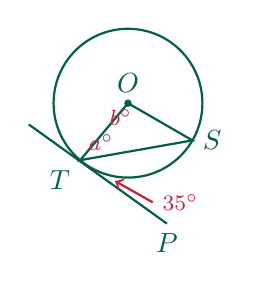
\begin{tikzpicture}[scale=0.90]
      \draw[thick, color=brandNavy] (0,0) circle (1.05);
      \coordinate (O) at (0,0);
      \coordinate (T) at (-130:1.05);
      \coordinate (S) at (-30:1.05);
      \coordinate (P) at (0.55, -1.7);
      \draw[thick, color=brandNavy] (O) node[above] {$O$} -- (T) node[below left] {$T$} -- (S) node[right] {$S$} -- cycle;
      \draw[thick, color=brandNavy] (-1.4, -0.3) -- (P) node[below] {$P$};
      \node[color=brandCrimson] at (-0.1, -0.2) {\footnotesize $b^\circ$};
      \node[color=brandCrimson] at (-0.38, -0.55) {\footnotesize $a^\circ$};
      \draw[->, color=brandCrimson, thick] (0.35, -1.4) -- (-0.18, -1.1);
      \node[right, color=brandCrimson] at (0.35, -1.4) {\footnotesize $35^\circ$};
      \fill[brandNavy] (O) circle (1.5pt);
    \end{tikzpicture}
  \end{khcard}
\end{minipage}\hfill
\begin{minipage}[t]{0.32\textwidth}
  \begin{khcard}
    \centering
    \alphabadge{ច} ចូររកតម្លៃនៃមុំ $a$ និង $b$\\[4pt]
    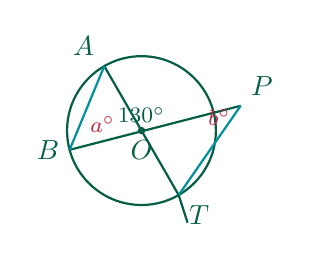
\begin{tikzpicture}[scale=0.90]
      \draw[thick, color=brandNavy] (0,0) circle (1.05);
      \coordinate (O) at (0,0);
      \coordinate (A) at (120:1.05);
      \coordinate (T) at (-60:1.05);
      \coordinate (B) at (195:1.05);
      \coordinate (P) at (1.4, 0.35);
      \draw[thick, color=brandNavy] (A) node[above left] {$A$} -- (T) node[below right] {$T$};
      \draw[thick, color=brandNavy] (B) node[left] {$B$} -- (P) node[above right] {$P$};
      \draw[thick, color=brandBlue] (A) -- (B);
      \draw[thick, color=brandBlue] (T) -- (P);
      \draw[thick, color=brandNavy] (0.65, -1.3) -- (T);
      \node[color=brandNavy] at (0.0, 0.22) {\footnotesize $130^\circ$};
      \node[color=brandCrimson] at (-0.55, 0.08) {\footnotesize $a^\circ$};
      \node[color=brandCrimson] at (1.1, 0.18) {\footnotesize $b^\circ$};
      \fill[brandNavy] (O) circle (1.5pt) node[below] {$O$};
    \end{tikzpicture}
  \end{khcard}
\end{minipage}

\vspace{6pt}
\begin{khboxpractice}
\begin{minipage}[c]{0.70\textwidth}
  \phead\ គេមានរង្វង់មួយដែលមានផ្ចិត $O$ និងកាំស្មើនឹង $2\text{cm}$ ។ $A$ ជាចំណុចមួយនៅក្រៅរង្វង់។ ពីចំណុច $A$ គេគូសបន្ទាត់ប៉ះនឹងរង្វង់ត្រង់ចំណុច $B$ និងបន្ទាត់មួយទៀតកាត់តាមផ្ចិត $O$ និងកាត់រង្វង់ត្រង់ $C$ ។ បើគេដឹងថា $AB = OB$ ចូរគណនារង្វាស់ $AC$ ។
\end{minipage}\hfill
\begin{minipage}[c]{0.28\textwidth}
  \centering
  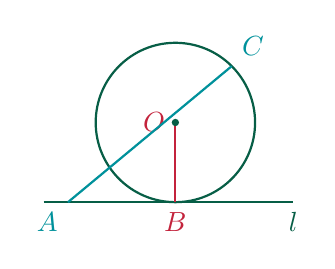
\begin{tikzpicture}[scale=0.88]
    \draw[thick, color=brandNavy] (0,0) circle (1.15);
    \coordinate (O) at (0,0);
    \coordinate (B) at (0,-1.15);
    \coordinate (A) at (-1.55,-1.15);
    \coordinate (C) at (45:1.15);
    \draw[thick, color=brandNavy] (-1.9,-1.15) -- (1.7,-1.15) node[below] {$l$};
    \draw[thick, color=brandCrimson] (O) node[left] {$O$} -- (B) node[below] {$B$};
    \draw[thick, color=brandBlue] (A) node[below left] {$A$} -- (C) node[above right] {$C$};
    \fill[brandNavy] (O) circle (1.5pt);
  \end{tikzpicture}
\end{minipage}
\end{khboxpractice}

\vspace{6pt}
% -------------------------------------------------------------------------
% SECTION 3 (TANGENT PROPERTIES)

\khsection{៣}{លក្ខណៈនៃបន្ទាត់ប៉ះ}

\begin{khboxmagenta}
  \textbf{បើបន្ទាត់ប៉ះរង្វង់ស្របទៅនឹងអង្កត់ធ្នូមួយនោះ ចំណុចប៉ះចែកធ្នូសន្ធឹងជាពីរផ្នែកប៉ុនគ្នា ។}
\end{khboxmagenta}

\vspace{3pt}
\begin{khcard}
\begin{minipage}[c]{0.68\textwidth}
  គេឲ្យបន្ទាត់ $EF$ ប៉ះរង្វង់ផ្ចិត $O$ ត្រង់ចំណុច $C$ ដែលមាន $AB \parallel EF$ ។\\
  ស្រាយបំភ្លឺថា $\wideparen{AC} = \wideparen{BC}$ ។
\end{minipage}\hfill
\begin{minipage}[c]{0.30\textwidth}
  \centering
  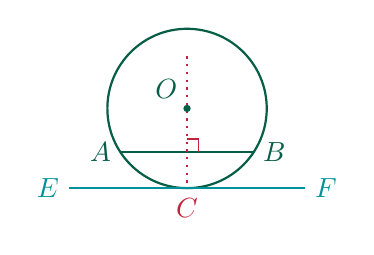
\begin{tikzpicture}[scale=0.88]
    \draw[thick, color=brandNavy] (0,0) circle (1.15);
    \coordinate (O) at (0,0);
    \coordinate (C) at (0,-1.15);
    \coordinate (A) at (-0.95,-0.63);
    \coordinate (B) at (0.95,-0.63);
    \draw[thick, color=brandNavy] (A) node[left] {$A$} -- (B) node[right] {$B$};
    \draw[thick, color=brandBlue] (-1.7,-1.15) node[left] {$E$} -- (1.7,-1.15) node[right] {$F$};
    \draw[thick, dotted, color=brandCrimson] (0,0.75) -- (C) node[below] {$C$};
    \fill[brandNavy] (O) circle (1.5pt) node[above left] {$O$};
    \draw[color=brandCrimson] (0,-0.44) -| (0.16,-0.63);
  \end{tikzpicture}
\end{minipage}
\end{khcard}

\vspace{3pt}
\begin{khcard}
\begin{minipage}[c]{0.65\textwidth}
  \exhead{} គេឲ្យបន្ទាត់ពីរ $AB$ និង $CD$ ប៉ះរង្វង់ផ្ចិត $O$ ត្រង់ចំណុចរៀង $B$ និង $C$ ។ ស្រាយបំភ្លឺថា ៖
  \begin{itemize}[leftmargin=15pt, itemsep=2pt]
    \item[\alphabadge{ក}] $AB = AC$
    \item[\alphabadge{ខ}] $\angle BAO = \angle OAC$
    \item[\alphabadge{គ}] $\angle BOA = \angle AOC$
    \item[\alphabadge{ឃ}] $\angle OBA = \angle OCA$
  \end{itemize}
\end{minipage}\hfill
\begin{minipage}[c]{0.33\textwidth}
  \centering
  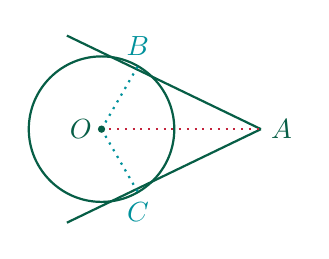
\begin{tikzpicture}[scale=0.88]
    \draw[thick, color=brandNavy] (0,0) circle (1.05);
    \coordinate (O) at (0,0);
    \coordinate (A) at (2.3,0);
    \coordinate (B) at (60:1.05);
    \coordinate (C) at (-60:1.05);
    \draw[thick, color=brandNavy] (-0.5, 1.35) -- (A) node[right] {$A$};
    \draw[thick, color=brandNavy] (-0.5, -1.35) -- (A);
    \draw[thick, dotted, color=brandCrimson] (O) -- (A);
    \draw[thick, dotted, color=brandBlue] (O) -- (B) node[above] {$B$};
    \draw[thick, dotted, color=brandBlue] (O) -- (C) node[below] {$C$};
    \fill[brandNavy] (O) circle (1.5pt) node[left] {$O$};
  \end{tikzpicture}
\end{minipage}
\end{khcard}

\vspace{3pt}
\begin{khboxmagenta}
  \begin{minipage}[c]{0.68\textwidth}
    បើបន្ទាត់ពីរគូសចេញពីចំណុចរួមមួយនៅក្រៅរង្វង់ហើយប៉ះរង្វង់នេះត្រង់ចំណុច $B$ និង $C$ គេបាន
    \begin{enumerate}[label=\protect\secbadge{\arabic*}, leftmargin=15pt, itemsep=2pt, topsep=1pt]
      \item បន្ទាត់ប៉ះនៃរង្វង់កែងទៅនឹងកាំត្រង់ចំណុចប៉ះ $\angle OBA = \angle OCA = 90^\circ$
      \item បន្ទាត់ប៉ះពីរទៅនឹងរង្វង់ដែលគូសចេញពីចំណុចរួមមួយនៅក្រៅរង្វង់មានប្រវែងស្មើគ្នា $AB = AC$
      \item បន្ទាត់ដែលគូសចេញពីចំណុចក្រៅរង្វង់មុំឈមទៅផ្ចិតនៃរង្វង់ ជាកន្លះបន្ទាត់ពុះនៃមុំឈមដែលផ្គុំដោយបន្ទាត់ប៉ះទាំងពីរ និងមុំដែលផ្គុំដោយកាំនៃរង្វង់ ៖
      \begin{itemize}[leftmargin=10pt, itemsep=1pt]
        \item $\angle OAB = \angle OAC$
        \item $\angle COA = \angle BOA$
      \end{itemize}
    \end{enumerate}
  \end{minipage}\hfill
  \begin{minipage}[c]{0.28\textwidth}
    \centering
    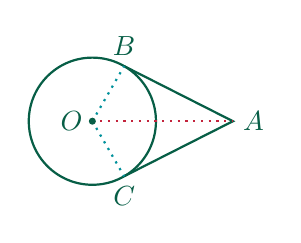
\begin{tikzpicture}[scale=0.85]
      \draw[thick, color=brandNavy] (0,0) circle (0.95);
      \coordinate (O) at (0,0);
      \coordinate (A) at (2.1,0);
      \coordinate (B) at (60:0.95);
      \coordinate (C) at (-60:0.95);
      \draw[thick, color=brandNavy] (B) node[above] {$B$} -- (A) node[right] {$A$} -- (C) node[below] {$C$};
      \draw[thick, dotted, color=brandCrimson] (O) -- (A);
      \draw[thick, dotted, color=brandBlue] (O) -- (B);
      \draw[thick, dotted, color=brandBlue] (O) -- (C);
      \fill[brandNavy] (O) circle (1.5pt) node[left] {$O$};
    \end{tikzpicture}
  \end{minipage}
\end{khboxmagenta}

\vspace{3pt}
\begin{khcard}
\begin{minipage}[c]{0.68\textwidth}
  \exhead{១} $O$ ជាផ្ចិតនៃរង្វង់មួយ (ដូចរូបខាងស្ដាំ) ។ $PA$ និង $PB$ ជាបន្ទាត់ប៉ះទៅនឹងរង្វង់ ។ បើ $\angle ABP = 63^\circ$ ។ ចូរគណនា $\angle AOB$ និង $\angle AOP$ ។
\end{minipage}\hfill
\begin{minipage}[c]{0.30\textwidth}
  \centering
  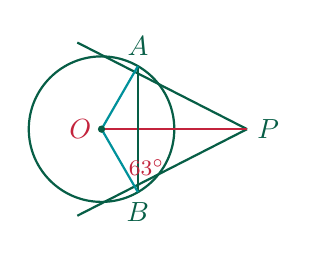
\begin{tikzpicture}[scale=0.88]
    \draw[thick, color=brandNavy] (0,0) circle (1.05);
    \coordinate (O) at (0,0);
    \coordinate (P) at (2.1,0);
    \coordinate (A) at (60:1.05);
    \coordinate (B) at (-60:1.05);
    \draw[thick, color=brandNavy] (-0.35, 1.25) -- (P) node[right] {$P$};
    \draw[thick, color=brandNavy] (-0.35, -1.25) -- (P);
    \draw[thick, color=brandCrimson] (O) node[left] {$O$} -- (P);
    \draw[thick, color=brandNavy] (A) node[above] {$A$} -- (B) node[below] {$B$};
    \draw[thick, color=brandBlue] (O) -- (A);
    \draw[thick, color=brandBlue] (O) -- (B);
    \node[color=brandCrimson] at (0.65, -0.55) {\footnotesize $63^\circ$};
    \fill[brandNavy] (O) circle (1.5pt);
  \end{tikzpicture}
\end{minipage}
\end{khcard}

\vspace{6pt}
% -------------------------------------------------------------------------
% EXERCISES 1 TO 4

\begin{khcard}
\begin{minipage}[c]{0.68\textwidth}
  \exhead{២} $TA$ និង $TB$ ជាបន្ទាត់ប៉ះទៅនឹងរង្វង់ផ្ចិត $O$ ដែលមានកាំ $9\text{cm}$ ។ បើ $\angle ATB = 110^\circ$ ។ ចូរគណនា
  \begin{itemize}[leftmargin=15pt, itemsep=2pt]
    \item[\alphabadge{ក}] $\angle AOB$
    \item[\alphabadge{ខ}] ផ្ទៃក្រឡាចម្រៀកថាសតូច $AOB$ ដែល $\pi = \dfrac{22}{7}$
  \end{itemize}
\end{minipage}\hfill
\begin{minipage}[c]{0.30\textwidth}
  \centering
  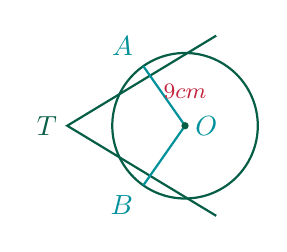
\begin{tikzpicture}[scale=0.88]
    \draw[thick, color=brandNavy] (0,0) circle (1.05);
    \coordinate (O) at (0,0);
    \coordinate (T) at (-1.7,0);
    \coordinate (A) at (125:1.05);
    \coordinate (B) at (-125:1.05);
    \draw[thick, color=brandNavy] (0.45, 1.3) -- (T) node[left] {$T$} -- (0.45, -1.3);
    \draw[thick, color=brandBlue] (O) node[right] {$O$} -- (A) node[above left] {$A$};
    \draw[thick, color=brandBlue] (O) -- (B) node[below left] {$B$};
    \node[above right, color=brandCrimson] at (-0.45, 0.25) {\footnotesize $9\text{cm}$};
    \fill[brandNavy] (O) circle (1.5pt);
  \end{tikzpicture}
\end{minipage}
\end{khcard}

\vspace{3pt}
\begin{khboxpractice}
  \phead\ $ST$ និង $RT$ ជាបន្ទាត់ប៉ះទៅនឹងរង្វង់មួយមានផ្ចិត $O$ ដែល $ST = RT = 20\text{cm}$ ។\\
  បើ $TQO$ ជាបន្ទាត់ត្រង់មួយដែល $TQ = 10\text{cm}$ ។ ចូរគណនាកាំនៃរង្វង់ $OQ$ ។
\end{khboxpractice}

\vspace{3pt}
\begin{khcard}
\begin{minipage}[c]{0.68\textwidth}
  \exerhead{១} នៅក្នុងរូបខាងស្ដាំនេះមាន $O$ ជាផ្ចិតនៃរង្វង់ហើយ $PA$ និង $PB$ ជាបន្ទាត់ប៉ះទៅនឹងរង្វង់រៀងគ្នាត្រង់ $A$ និង $B$ រង្វាស់គិតជា $\text{cm}$ ។ ចូរគណនា
  \begin{itemize}[leftmargin=15pt, itemsep=1.5pt]
    \item[\alphabadge{ក}] រង្វាស់ $b$
    \item[\alphabadge{ខ}] រង្វាស់ $c$
    \item[\alphabadge{គ}] បរិមាត្រនៃចតុកោណ $OAPB$
    \item[\alphabadge{ឃ}] ផ្ទៃក្រឡានៃចតុកោណ $OAPB$
  \end{itemize}
\end{minipage}\hfill
\begin{minipage}[c]{0.30\textwidth}
  \centering
  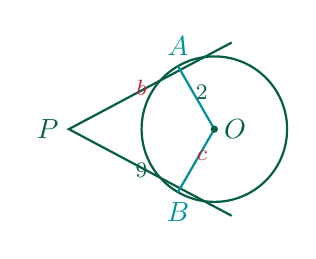
\begin{tikzpicture}[scale=0.88]
    \draw[thick, color=brandNavy] (0,0) circle (1.05);
    \coordinate (O) at (0,0);
    \coordinate (P) at (-2.1,0);
    \coordinate (A) at (120:1.05);
    \coordinate (B) at (-120:1.05);
    \draw[thick, color=brandNavy] (0.25, 1.25) -- (P) node[left] {$P$} -- (0.25, -1.25);
    \draw[thick, color=brandBlue] (O) -- (A) node[above] {$A$};
    \draw[thick, color=brandBlue] (O) -- (B) node[below] {$B$};
    \fill[brandNavy] (O) circle (1.5pt) node[right] {$O$};
    \node[above, color=brandCrimson] at (-1.05, 0.35) {\footnotesize $b$};
    \node[below, color=brandNavy] at (-1.05, -0.35) {\footnotesize $9$};
    \node[above, color=brandNavy] at (-0.18, 0.28) {\footnotesize $2$};
    \node[below, color=brandCrimson] at (-0.18, -0.18) {\footnotesize $c$};
  \end{tikzpicture}
\end{minipage}
\end{khcard}

\vspace{3pt}
\begin{khcard}
\begin{minipage}[c]{0.68\textwidth}
  \exerhead{២} គេមាន $PA$ និង $PB$ ជាបន្ទាត់ប៉ះទៅនឹងរង្វង់ដែលមានផ្ចិត $O$ និងកាំ $3\text{cm}$ ។ គេឲ្យ $AP = 82.4\text{cm}$ និង $\angle AOB = 140^\circ$ ។ ចូរគណនាផ្ទៃក្រឡានៃ ៖
  \begin{itemize}[leftmargin=15pt, itemsep=1.5pt]
    \item[\alphabadge{ក}] ចតុកោណ $APBO$
    \item[\alphabadge{ខ}] ចម្រៀកថាសតូច $AOB$ យក $(\pi = \dfrac{22}{7})$
  \end{itemize}
\end{minipage}\hfill
\begin{minipage}[c]{0.30\textwidth}
  \centering
  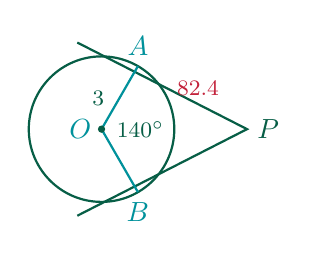
\begin{tikzpicture}[scale=0.88]
    \draw[thick, color=brandNavy] (0,0) circle (1.05);
    \coordinate (O) at (0,0);
    \coordinate (P) at (2.1,0);
    \coordinate (A) at (60:1.05);
    \coordinate (B) at (-60:1.05);
    \draw[thick, color=brandNavy] (-0.35, 1.25) -- (P) node[right] {$P$} -- (-0.35, -1.25);
    \draw[thick, color=brandBlue] (O) node[left] {$O$} -- (A) node[above] {$A$};
    \draw[thick, color=brandBlue] (O) -- (B) node[below] {$B$};
    \fill[brandNavy] (O) circle (1.5pt);
    \node[left, color=brandNavy] at (0.18, 0.45) {\footnotesize $3$};
    \node[above right, color=brandCrimson] at (0.95, 0.35) {\footnotesize $82.4$};
    \node[right, color=brandNavy] at (0.08, 0) {\footnotesize $140^\circ$};
  \end{tikzpicture}
\end{minipage}
\end{khcard}

\vspace{3pt}
\begin{khcard}
\begin{minipage}[c]{0.68\textwidth}
  \exerhead{៣} ក្នុងរង្វង់ផ្ចិត $O$ គេមាន $AT$ និង $BT$ មានប្រវែង $20\text{cm}$ ។ បើ $TQO$ ជាបន្ទាត់ត្រង់ដែល $TQ = 10\text{cm}$ ។ ចូររករង្វាស់នៃកាំរង្វង់ ។
\end{minipage}\hfill
\begin{minipage}[c]{0.30\textwidth}
  \centering
  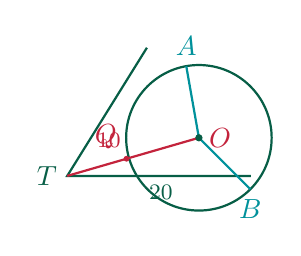
\begin{tikzpicture}[scale=0.88]
    \draw[thick, color=brandNavy] (0,0) circle (1.05);
    \coordinate (O) at (0,0);
    \coordinate (T) at (-1.9, -0.55);
    \coordinate (A) at (100:1.05);
    \coordinate (B) at (-45:1.05);
    \draw[thick, color=brandNavy] (-0.75, 1.3) -- (T) node[left] {$T$} -- (0.75, -0.55);
    \draw[thick, color=brandCrimson] (T) -- (O) node[right] {$O$};
    \draw[thick, color=brandBlue] (O) -- (A) node[above] {$A$};
    \draw[thick, color=brandBlue] (O) -- (B) node[below] {$B$};
    \fill[brandNavy] (O) circle (1.5pt);
    \fill[brandCrimson] ($(T)!0.45!(O)$) circle (1.2pt) node[above left] {$Q$};
    \node[above, color=brandCrimson] at (-1.3, -0.28) {\footnotesize $10$};
    \node[below, color=brandNavy] at (-0.55, -0.55) {\footnotesize $20$};
  \end{tikzpicture}
\end{minipage}
\end{khcard}

\vspace{3pt}
\begin{khcard}
\begin{minipage}[c]{0.68\textwidth}
  \exerhead{៤} នៅក្នុងរង្វង់ផ្ចិត $O$ ដែលមានកាំ $4.5\text{cm}$ ។ គេមាន $TA$ និង $TB$ ជាបន្ទាត់ប៉ះនឹងរង្វង់រៀងគ្នាត្រង់ $A$ និង $B$ ដែល $TA = 9\text{cm}$ ។
  \begin{itemize}[leftmargin=15pt, itemsep=1.5pt]
    \item[\alphabadge{ក}] គណនាបរិមាត្រនៃចតុកោណ $OATB$
    \item[\alphabadge{ខ}] គណនាផ្ទៃក្រឡានៃចតុកោណ $OATB$
  \end{itemize}
\end{minipage}\hfill
\begin{minipage}[c]{0.30\textwidth}
  \centering
  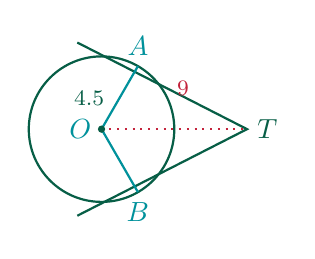
\begin{tikzpicture}[scale=0.88]
    \draw[thick, color=brandNavy] (0,0) circle (1.05);
    \coordinate (O) at (0,0);
    \coordinate (T) at (2.1,0);
    \coordinate (A) at (60:1.05);
    \coordinate (B) at (-60:1.05);
    \draw[thick, color=brandNavy] (-0.35, 1.25) -- (T) node[right] {$T$} -- (-0.35, -1.25);
    \draw[thick, dotted, color=brandCrimson] (O) -- (T);
    \draw[thick, color=brandBlue] (O) node[left] {$O$} -- (A) node[above] {$A$};
    \draw[thick, color=brandBlue] (O) -- (B) node[below] {$B$};
    \fill[brandNavy] (O) circle (1.5pt);
    \node[left, color=brandNavy] at (0.18, 0.45) {\footnotesize $4.5$};
    \node[above right, color=brandCrimson] at (0.95, 0.35) {\footnotesize $9$};
  \end{tikzpicture}
\end{minipage}
\end{khcard}

\vspace{6pt}
% -------------------------------------------------------------------------
% CIRCUMSCRIBED QUADRILATERALS

\khsection{៤}{អនុវត្តន៍លក្ខណៈជ្រុងឈមនៃចតុកោណចារឹកក្រៅរង្វង់}

\vspace{3pt}
\begin{khcard}
\begin{minipage}[c]{0.65\textwidth}
  \exhead{} នៅក្នុងចតុកោណ $ABCD$ ដូចរូបខាងស្ដាំ\\
  ជ្រុងទាំងបួនជាបន្ទាត់ប៉ះរង្វង់ត្រង់ $P, Q, R$ និង $S$ ។\\
  ចតុកោណ $ABCD$ ដែលមានជ្រុងទាំងបួនប៉ះរង្វង់តែមួយ ហៅថា\textbf{\color{brandNavy}ចតុកោណចារឹកក្រៅរង្វង់} ។ បង្ហាញថា ៖
  \begin{itemize}[leftmargin=15pt, itemsep=2pt]
    \item[\alphabadge{ក}] $AP = AS, BP = BQ, CQ = CR$ និង $DR = DS$
    \item[\alphabadge{ខ}] $AB + CD = AD + BC$
  \end{itemize}
\end{minipage}\hfill
\begin{minipage}[c]{0.33\textwidth}
  \centering
  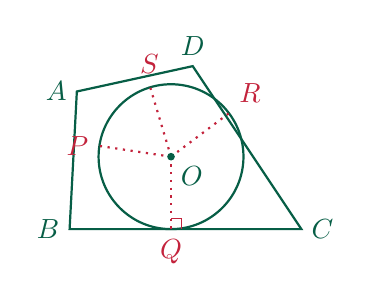
\begin{tikzpicture}[scale=0.92]
    \draw[thick, color=brandNavy] (0,0) circle (1.0);
    \coordinate (O) at (0,0);
    \coordinate (A) at (-1.3, 0.9);
    \coordinate (B) at (-1.4, -1.0);
    \coordinate (C) at (1.8, -1.0);
    \coordinate (D) at (0.3, 1.25);
    \draw[thick, color=brandNavy] (A) node[left] {$A$} -- (D) node[above] {$D$} -- (C) node[right] {$C$} -- (B) node[left] {$B$} -- cycle;
    \coordinate (P) at (-1.0, 0.15);
    \coordinate (Q) at (0.0, -1.0);
    \coordinate (R) at (0.8, 0.6);
    \coordinate (S) at (-0.3, 1.0);
    \draw[thick, dotted, color=brandCrimson] (O) -- (P) node[left] {$P$};
    \draw[thick, dotted, color=brandCrimson] (O) -- (Q) node[below] {$Q$};
    \draw[thick, dotted, color=brandCrimson] (O) -- (R) node[above right] {$R$};
    \draw[thick, dotted, color=brandCrimson] (O) -- (S) node[above] {$S$};
    \fill[brandNavy] (O) circle (1.5pt) node[below right] {$O$};
    \draw[color=brandCrimson] (0, -0.85) -| (0.15, -1.0);
  \end{tikzpicture}
\end{minipage}

\vspace{3pt}
\begin{center}
  \textbf{\color{brandCrimson}\kml ស្រាយបញ្ជាក់}\\[2pt]
  \dotfill
\end{center}
\end{khcard}

\vspace{4pt}
\begin{khboxmagenta}
  \textbf{ក្នុងចតុកោណចារឹកក្រៅរង្វង់ ផលបូករង្វាស់ជ្រុងឈមមានរង្វាស់ស្មើគ្នា ៖}
  \begin{equation*}
    AB + CD = AD + BC
  \end{equation*}
\end{khboxmagenta}

\vspace{4pt}
\begin{khcard}
  \samplehead\ រង្វង់ផ្ចិត $O$ ប៉ះនឹងជ្រុងទាំងបួននៃចតុកោណ $ABCD$ ដែល $AB = 20\text{cm}, CD = 14\text{cm}$ និង $BC = 11\text{cm}$ ។ ចូរគណនារង្វាស់ $AD$ ។
\end{khcard}

\vspace{4pt}
\begin{khboxpractice}
\begin{minipage}[c]{0.68\textwidth}
  \phead\ ក្នុងរូបខាងស្ដាំនេះ $ABC$ ជាត្រីកោណសមបាតដែលមានកំពូល $A$ ។ ចូរស្រាយបំភ្លឺថា $BR = RC$ ។
\end{minipage}\hfill
\begin{minipage}[c]{0.30\textwidth}
  \centering
  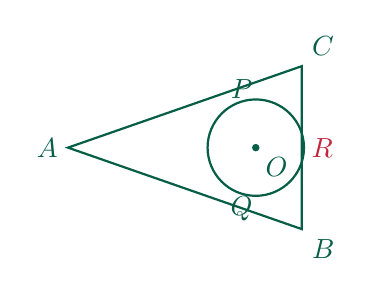
\begin{tikzpicture}[scale=0.90]
    \coordinate (A) at (-1.9,0);
    \coordinate (B) at (1.4,-1.15);
    \coordinate (C) at (1.4,1.15);
    \draw[thick, color=brandNavy] (A) node[left] {$A$} -- (B) node[below right] {$B$} -- (C) node[above right] {$C$} -- cycle;
    \draw[thick, color=brandTeal] (0.75,0) circle (0.68);
    \fill[brandNavy] (0.75,0) circle (1.5pt) node[below right] {$O$};
    \node[above, color=brandTeal] at (0.55, 0.55) {$P$};
    \node[below, color=brandTeal] at (0.55, -0.55) {$Q$};
    \node[right, color=brandCrimson] at (1.4, 0) {$R$};
  \end{tikzpicture}
\end{minipage}
\end{khboxpractice}

\vspace{4pt}
\begin{khcard}
\begin{minipage}[c]{0.68\textwidth}
  \exhead{} រង្វង់ពីរមានផ្ចិតរួម $O$ មានកាំ $8\text{cm}$ និង $10\text{cm}$ ។ $AB$ ជាអង្កត់ធ្នូនរង្វង់ធំហើយប៉ះរង្វង់តូចត្រង់ $T$ ។ ចូរគណនា $AB$ ។ ( \textbf{ណែនាំ} ៖ គូស $OA$ និង $OB$ )
\end{minipage}\hfill
\begin{minipage}[c]{0.30\textwidth}
  \centering
  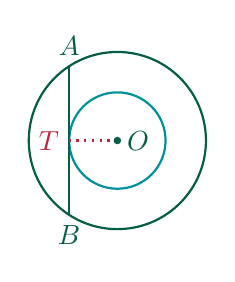
\begin{tikzpicture}[scale=0.90]
    \draw[thick, color=brandNavy] (0,0) circle (1.25);
    \draw[thick, color=brandBlue] (0,0) circle (0.68);
    \coordinate (O) at (0,0);
    \coordinate (T) at (-0.68,0);
    \coordinate (A) at (-0.68, 1.05);
    \coordinate (B) at (-0.68, -1.05);
    \draw[thick, color=brandNavy] (A) node[above] {$A$} -- (B) node[below] {$B$};
    \draw[thick, dotted, color=brandCrimson] (O) -- (T) node[left] {$T$};
    \fill[brandNavy] (O) circle (1.5pt) node[right] {$O$};
  \end{tikzpicture}
\end{minipage}
\end{khcard}

\vspace{6pt}
% -------------------------------------------------------------------------
% RELATIVE POSITIONS OF TWO CIRCLES

\khsection{៥}{ទីតាំងរង្វង់}

គេមានរង្វង់ពីរដែលមានផ្ចិត $O$ និង $O'$ និងកាំរៀងគ្នា $r$ និង $r'$ ។ ហើយ $d$ ជាចម្ងាយរវាងផ្ចិតទាំងពីរ ដូចរូបខាងក្រោម ៖

\vspace{4pt}
% 5 Cases Grid in clean cards
\begin{minipage}[t]{0.48\textwidth}
  \begin{khcard}
    \centering
    \secbadge{1} \textcolor{brandCrimson}{\textbf{$d > r + r'$}}\\[2pt]
    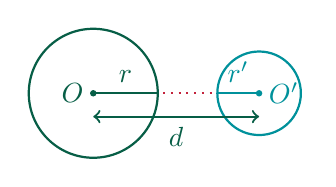
\begin{tikzpicture}[scale=0.78]
      \draw[thick, color=brandNavy] (0,0) circle (1.05);
      \draw[thick, color=brandBlue] (2.7,0) circle (0.68);
      \coordinate (O) at (0,0);
      \coordinate (O1) at (2.7,0);
      \draw[thick, dotted, color=brandCrimson] (O) -- (O1);
      \draw[<->, thick, color=brandNavy] (0,-0.38) -- (2.7,-0.38) node[midway, below] {$d$};
      \draw[thick, color=brandNavy] (O) -- ++(1.05,0) node[midway, above] {$r$};
      \draw[thick, color=brandBlue] (O1) -- ++(-0.68,0) node[midway, above] {$r'$};
      \fill[brandNavy] (O) circle (1.5pt) node[left] {$O$};
      \fill[brandBlue] (O1) circle (1.5pt) node[right] {$O'$};
    \end{tikzpicture}\\[2pt]
    \textbf{\color{brandNavy}រង្វង់គ្មានចំណុចរួម}
  \end{khcard}
\end{minipage}\hfill
\begin{minipage}[t]{0.48\textwidth}
  \begin{khcard}
    \centering
    \secbadge{2} \textcolor{brandCrimson}{\textbf{$d = r + r'$}}\\[2pt]
    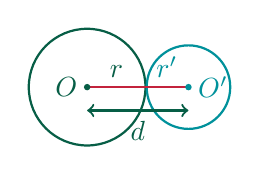
\begin{tikzpicture}[scale=0.78]
      \draw[thick, color=brandNavy] (0,0) circle (0.95);
      \draw[thick, color=brandBlue] (1.65,0) circle (0.68);
      \coordinate (O) at (0,0);
      \coordinate (O1) at (1.65,0);
      \draw[thick, color=brandCrimson] (O) -- (O1);
      \draw[<->, thick, color=brandNavy] (0,-0.38) -- (1.65,-0.38) node[midway, below] {$d$};
      \node[above, color=brandNavy] at (0.48,0) {$r$};
      \node[above, color=brandBlue] at (1.3,0) {$r'$};
      \fill[brandNavy] (O) circle (1.5pt) node[left] {$O$};
      \fill[brandBlue] (O1) circle (1.5pt) node[right] {$O'$};
    \end{tikzpicture}\\[2pt]
    \textbf{\color{brandNavy}រង្វង់មានចំណុចរួមមួយ (ប៉ះក្រៅ)}
  \end{khcard}
\end{minipage}

\vspace{4pt}
\begin{minipage}[t]{0.32\textwidth}
  \begin{khcard}
    \centering
    \secbadge{3} \textcolor{brandCrimson}{\textbf{\footnotesize $r-r' < d < r+r'$}}\\[2pt]
    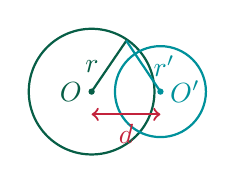
\begin{tikzpicture}[scale=0.76]
      \draw[thick, color=brandNavy] (0,0) circle (1.05);
      \draw[thick, color=brandBlue] (1.15,0) circle (0.76);
      \coordinate (O) at (0,0);
      \coordinate (O1) at (1.15,0);
      \coordinate (P) at (0.58,0.85);
      \draw[thick, color=brandNavy] (O) -- (P) node[midway, left] {$r$};
      \draw[thick, color=brandBlue] (O1) -- (P) node[midway, right] {$r'$};
      \draw[<->, thick, color=brandCrimson] (0,-0.38) -- (1.15,-0.38) node[midway, below] {$d$};
      \fill[brandNavy] (O) circle (1.5pt) node[left] {$O$};
      \fill[brandBlue] (O1) circle (1.5pt) node[right] {$O'$};
    \end{tikzpicture}\\[2pt]
    \textbf{\footnotesize\color{brandNavy} រង្វង់កាត់គ្នាពីរចំណុច}
  \end{khcard}
\end{minipage}\hfill
\begin{minipage}[t]{0.32\textwidth}
  \begin{khcard}
    \centering
    \secbadge{4} \textcolor{brandCrimson}{\textbf{$d = r - r'$}}\\[2pt]
    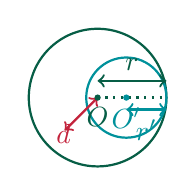
\begin{tikzpicture}[scale=0.76]
      \draw[thick, color=brandNavy] (0,0) circle (1.15);
      \draw[thick, color=brandBlue] (0.48,0) circle (0.67);
      \coordinate (O) at (0,0);
      \coordinate (O1) at (0.48,0);
      \draw[thick, dotted, color=brandNavy] (O) -- (1.15,0);
      \draw[<->, thick, color=brandNavy] (0,0.28) -- (1.15,0.28) node[midway, above] {$r$};
      \draw[<->, thick, color=brandBlue] (0.48,-0.2) -- (1.15,-0.2) node[midway, below] {$r'$};
      \draw[<->, thick, color=brandCrimson] (O) -- ++(-0.55,-0.55) node[midway, below left] {$d$};
      \fill[brandNavy] (O) circle (1.5pt) node[below] {$O$};
      \fill[brandBlue] (O1) circle (1.5pt) node[below] {$O'$};
    \end{tikzpicture}\\[2pt]
    \textbf{\footnotesize\color{brandNavy} រង្វង់ប៉ះក្នុង}
  \end{khcard}
\end{minipage}\hfill
\begin{minipage}[t]{0.32\textwidth}
  \begin{khcard}
    \centering
    \secbadge{5} \textcolor{brandCrimson}{\textbf{$d < r - r'$}}\\[2pt]
    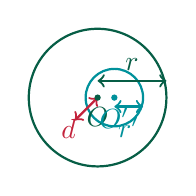
\begin{tikzpicture}[scale=0.76]
      \draw[thick, color=brandNavy] (0,0) circle (1.15);
      \draw[thick, color=brandBlue] (0.28,0) circle (0.48);
      \coordinate (O) at (0,0);
      \coordinate (O1) at (0.28,0);
      \draw[<->, thick, color=brandNavy] (0,0.28) -- (1.15,0.28) node[midway, above] {$r$};
      \draw[<->, thick, color=brandBlue] (0.28,-0.15) -- (0.76,-0.15) node[midway, below] {$r'$};
      \draw[<->, thick, color=brandCrimson] (O) -- ++(-0.38,-0.38) node[midway, below left] {$d$};
      \fill[brandNavy] (O) circle (1.5pt) node[below] {$O$};
      \fill[brandBlue] (O1) circle (1.5pt) node[below] {$O'$};
    \end{tikzpicture}\\[2pt]
    \textbf{\footnotesize\color{brandNavy} រង្វង់គ្មានចំណុចរួម}
  \end{khcard}
\end{minipage}

\vspace{3pt}
\begin{khcard}
  កាលណារង្វង់ពីរកាត់គ្នាត្រង់មួយចំណុចដូចរូប (2) និង រូប (4) គេថារង្វង់ទាំងពីរ\textbf{\color{brandCrimson}ប៉ះគ្នា} ។ ចំណុចប្រសព្វជាចំណុចប៉ះ។ ក្នុងករណីទាំងពីរនេះ ចំណុចប៉ះស្ថិតនៅលើបន្ទាត់កាត់ផ្ចិតនៃរង្វង់ទាំងពីរ ។\\
  ក្នុងរូបទី (2) គេថារង្វង់ប៉ះក្រៅនិងរូបទី (4) គេថារង្វង់ប៉ះក្នុង ។ រូបទី (3) ជាករណីដែលរង្វង់ពីរប្រសព្វគ្នា ។ ចំណុចប្រសព្វទាំងពីរឆ្លុះគ្នាធៀបនឹងបន្ទាត់ដែលកាត់តាមផ្ចិតនៃរង្វង់ទាំងពីរ ។
\end{khcard}

\vspace{3pt}
\begin{khcard}
  \exhead{} គេឲ្យរង្វង់ពីរដែលមានកាំរៀងគ្នា $r = 5\text{cm}, r' = 3\text{cm}$ ហើយ $OO'$ ជាចម្ងាយរវាងផ្ចិតទាំងពីរ ដែល $OO' = 2x + 1$ ។ ចូរកំណត់ $x$ ដើម្បីឲ្យ ៖
  \begin{itemize}[leftmargin=15pt, itemsep=1.5pt]
    \item[\alphabadge{ក}] រង្វង់ទាំងពីរប៉ះក្រៅ
    \item[\alphabadge{ខ}] រង្វង់ទាំងពីរប៉ះក្នុង
    \item[\alphabadge{គ}] រង្វង់កាត់គ្នាត្រង់ពីរចំណុច
  \end{itemize}
\end{khcard}

\vspace{3pt}
\begin{khboxpractice}
\begin{minipage}[c]{0.65\textwidth}
  \phead\ គេឲ្យរង្វង់ពីរដែលមានកាំរៀងគ្នា $r = 5\text{cm}$ និង $r' = 3\text{cm}$ ។\\
  $OO'$ កាត់រង្វង់រៀងគ្នាត្រង់ចំណុច $A$ និង $B$ ។ ចូរគណនាប្រវែង $AB$ ។
\end{minipage}\hfill
\begin{minipage}[c]{0.33\textwidth}
  \centering
  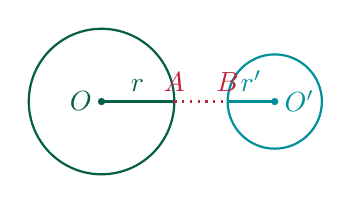
\begin{tikzpicture}[scale=0.88]
    \draw[thick, color=brandNavy] (0,0) circle (1.05);
    \draw[thick, color=brandBlue] (2.5,0) circle (0.68);
    \coordinate (O) at (0,0);
    \coordinate (O1) at (2.5,0);
    \coordinate (A) at (1.05,0);
    \coordinate (B) at (1.82,0);
    \draw[thick, color=brandNavy] (O) -- (A);
    \draw[thick, dotted, color=brandCrimson] (A) -- (B);
    \draw[thick, color=brandBlue] (B) -- (O1);
    \fill[brandNavy] (O) circle (1.5pt) node[left] {$O$};
    \fill[brandBlue] (O1) circle (1.5pt) node[right] {$O'$};
    \node[above, color=brandNavy] at (0.52,0) {$r$};
    \node[above, color=brandCrimson] at (A) {$A$};
    \node[above, color=brandCrimson] at (B) {$B$};
    \node[above, color=brandBlue] at (2.16,0) {$r'$};
  \end{tikzpicture}
\end{minipage}

\vspace{2pt}
\begin{center}
  \textbf{\color{brandCrimson}\kml ដំណោះស្រាយ}\\[2pt]
  \dotfill
\end{center}
\end{khboxpractice}

\vspace{6pt}
% -------------------------------------------------------------------------
% COMMON TANGENTS

\khsection{៦}{បន្ទាត់ប៉ះរួម}

បន្ទាត់ប៉ះរួមនៃរង្វង់ពីរផ្សេងគ្នាអាស្រ័យលើទំនាក់ទំនងទីតាំងនៃរង្វង់ទាំងពីរដូចរូបខាងក្រោម ៖

\vspace{3pt}
\begin{khcard}
\textbf{\fontsize{10}{10}\selectfont\kml\color{brandNavy} ក. រង្វង់គ្មានចំណុចរួម}

\vspace{1pt}
\begin{minipage}[c]{0.65\textwidth}
  \begin{itemize}[leftmargin=12pt, itemsep=1.5pt]
    \item[\color{brandBlue}\textbullet] រង្វង់ទាំងពីរគ្មានចំណុចរួម $AB$ និង $CD$ ហៅថា\textbf{\color{brandCrimson}បន្ទាត់ប៉ះរួមខាងក្រៅ} ។ រង្វង់ទាំងពីរស្ថិតនៅតែម្ខាងនៃបន្ទាត់ $AB$ និង $CD$ ។
  \end{itemize}
\end{minipage}\hfill
\begin{minipage}[c]{0.33\textwidth}
  \centering
  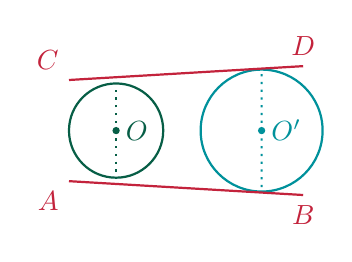
\begin{tikzpicture}[scale=0.88]
    \draw[thick, color=brandNavy] (0,0) circle (0.68);
    \draw[thick, color=brandBlue] (2.1,0) circle (0.88);
    \coordinate (O) at (0,0);
    \coordinate (O1) at (2.1,0);
    \draw[thick, color=brandCrimson] (-0.68, 0.73) node[above left] {$C$} -- (2.7, 0.93) node[above] {$D$};
    \draw[thick, color=brandCrimson] (-0.68, -0.73) node[below left] {$A$} -- (2.7, -0.93) node[below] {$B$};
    \draw[thick, dotted, color=brandNavy] (O) -- (0,0.68);
    \draw[thick, dotted, color=brandNavy] (O) -- (0,-0.68);
    \draw[thick, dotted, color=brandBlue] (O1) -- (2.1,0.88);
    \draw[thick, dotted, color=brandBlue] (O1) -- (2.1,-0.88);
    \fill[brandNavy] (O) circle (1.5pt) node[right] {$O$};
    \fill[brandBlue] (O1) circle (1.5pt) node[right] {$O'$};
  \end{tikzpicture}
\end{minipage}

\vspace{2pt}
\begin{minipage}[c]{0.65\textwidth}
  \begin{itemize}[leftmargin=12pt, itemsep=1.5pt]
    \item[\color{brandBlue}\textbullet] រង្វង់ទាំងពីរគ្មានចំណុចរួម បន្ទាត់ $MN$ និង $PQ$ ហៅថា\textbf{\color{brandCrimson}បន្ទាត់ប៉ះរួមខាងក្នុង} ។ រង្វង់ទាំងពីរស្ថិតនៅសងខាងនៃបន្ទាត់ $MN$ និង $PQ$ ។
  \end{itemize}
\end{minipage}\hfill
\begin{minipage}[c]{0.33\textwidth}
  \centering
  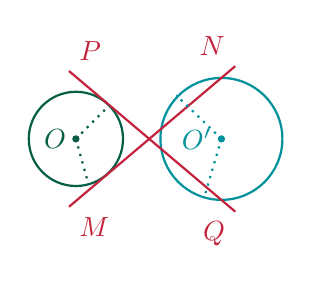
\begin{tikzpicture}[scale=0.88]
    \draw[thick, color=brandNavy] (0,0) circle (0.68);
    \draw[thick, color=brandBlue] (2.1,0) circle (0.88);
    \coordinate (O) at (0,0);
    \coordinate (O1) at (2.1,0);
    \draw[thick, color=brandCrimson] (-0.1, 0.98) node[above right] {$P$} -- (2.3, -1.05) node[below left] {$Q$};
    \draw[thick, color=brandCrimson] (-0.1, -0.98) node[below right] {$M$} -- (2.3, 1.05) node[above left] {$N$};
    \draw[thick, dotted, color=brandNavy] (O) -- (0.48, 0.48);
    \draw[thick, dotted, color=brandNavy] (O) -- (0.18, -0.65);
    \draw[thick, dotted, color=brandBlue] (O1) -- (1.45, 0.63);
    \draw[thick, dotted, color=brandBlue] (O1) -- (1.85, -0.85);
    \fill[brandNavy] (O) circle (1.5pt) node[left] {$O$};
    \fill[brandBlue] (O1) circle (1.5pt) node[left] {$O'$};
  \end{tikzpicture}
\end{minipage}
\end{khcard}

\vspace{3pt}
\begin{khcard}
\textbf{\fontsize{10}{10}\selectfont\kml\color{brandNavy} ខ. រង្វង់ប៉ះគ្នា}

\vspace{1pt}
\begin{minipage}[c]{0.65\textwidth}
  \begin{itemize}[leftmargin=12pt, itemsep=1.5pt]
    \item[\color{brandBlue}\textbullet] រង្វង់ពីរមានចំណុចរួមមួយ ហៅថារង្វង់ប៉ះគ្នា ។ $l$ ជាបន្ទាត់ប៉ះរួមដែលរង្វង់ទាំងពីរ ស្ថិតនៅសងខាងនៃបន្ទាត់ $l$ ។
  \end{itemize}
\end{minipage}\hfill
\begin{minipage}[c]{0.33\textwidth}
  \centering
  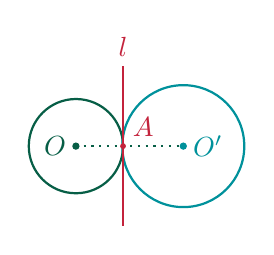
\begin{tikzpicture}[scale=0.88]
    \draw[thick, color=brandNavy] (0,0) circle (0.68);
    \draw[thick, color=brandBlue] (1.55,0) circle (0.88);
    \coordinate (O) at (0,0);
    \coordinate (O1) at (1.55,0);
    \draw[thick, color=brandCrimson] (0.68, 1.15) node[above] {$l$} -- (0.68, -1.15);
    \draw[thick, dotted, color=brandNavy] (O) -- (O1);
    \fill[brandNavy] (O) circle (1.5pt) node[left] {$O$};
    \fill[brandBlue] (O1) circle (1.5pt) node[right] {$O'$};
    \fill[brandCrimson] (0.68,0) circle (1.2pt) node[above right] {$A$};
  \end{tikzpicture}
\end{minipage}

\vspace{2pt}
\begin{minipage}[c]{0.65\textwidth}
  \begin{itemize}[leftmargin=12pt, itemsep=1.5pt]
    \item[\color{brandBlue}\textbullet] រង្វង់ទាំងពីរមានចំណុចរួមមួយ ។ $l$ ជាបន្ទាត់ប៉ះរួម ។ រង្វង់ទាំងពីរស្ថិតនៅតែម្ខាងនៃបន្ទាត់ $l$ ។
  \end{itemize}
\end{minipage}\hfill
\begin{minipage}[c]{0.33\textwidth}
  \centering
  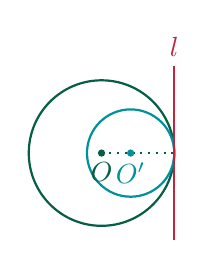
\begin{tikzpicture}[scale=0.88]
    \draw[thick, color=brandNavy] (0,0) circle (1.05);
    \draw[thick, color=brandBlue] (0.42,0) circle (0.63);
    \coordinate (O) at (0,0);
    \coordinate (O1) at (0.42,0);
    \draw[thick, color=brandCrimson] (1.05, 1.25) node[above] {$l$} -- (1.05, -1.25);
    \draw[thick, dotted, color=brandNavy] (O) -- (1.05,0);
    \fill[brandNavy] (O) circle (1.5pt) node[below] {$O$};
    \fill[brandBlue] (O1) circle (1.5pt) node[below] {$O'$};
  \end{tikzpicture}
\end{minipage}
\end{khcard}

\vspace{3pt}
\begin{khcard}
\textbf{\fontsize{10}{10}\selectfont\kml\color{brandNavy} គ. រង្វង់កាត់គ្នា}

\vspace{1pt}
\begin{minipage}[c]{0.65\textwidth}
  រង្វង់ទាំងពីរកាត់គ្នាត្រង់ពីរចំណុច ។ បន្ទាត់ $XY$ និង $ZE$ ជាបន្ទាត់ប៉ះរួមខាងក្រៅ ។ រង្វង់ទាំងពីរស្ថិតនៅតែម្ខាងនៃ $XY$ និង $ZE$ ។
\end{minipage}\hfill
\begin{minipage}[c]{0.33\textwidth}
  \centering
  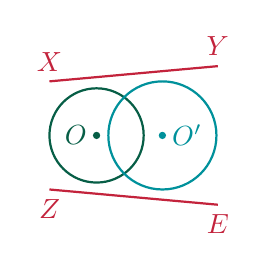
\begin{tikzpicture}[scale=0.88]
    \draw[thick, color=brandNavy] (0,0) circle (0.68);
    \draw[thick, color=brandBlue] (0.95,0) circle (0.78);
    \coordinate (O) at (0,0);
    \coordinate (O1) at (0.95,0);
    \draw[thick, color=brandCrimson] (-0.68, 0.78) node[above] {$X$} -- (1.75, 1.0) node[above] {$Y$};
    \draw[thick, color=brandCrimson] (-0.68, -0.78) node[below] {$Z$} -- (1.75, -1.0) node[below] {$E$};
    \fill[brandNavy] (O) circle (1.5pt) node[left] {$O$};
    \fill[brandBlue] (O1) circle (1.5pt) node[right] {$O'$};
  \end{tikzpicture}
\end{minipage}
\end{khcard}

\vspace{3pt}
\begin{khcard}
\textbf{\fontsize{10}{10}\selectfont\kml\color{brandNavy} ឃ. រង្វង់តូចនៅក្នុងរង្វង់ធំ}

\vspace{1pt}
\begin{minipage}[c]{0.65\textwidth}
  គ្មានចំណុចប៉ះរួម ។
\end{minipage}\hfill
\begin{minipage}[c]{0.33\textwidth}
  \centering
  
\begin{tikzpicture}[scale=0.88]
    \draw[thick, color=brandNavy] (0,0) circle (1.05);
    \draw[thick, color=brandBlue] (0.28,0.08) circle (0.52);
    \fill[brandNavy] (0,0) circle (1.5pt) node[below] {$O$};
    \fill[brandBlue] (0.28,0.08) circle (1.5pt) node[below] {$O'$};
  \end{tikzpicture}
\end{minipage}
\end{khcard}

\vspace{6pt}
% -------------------------------------------------------------------------
% EXERCISES, COMMON TANGENT TABLE & MOTTO

\samplehead\ គេមានរង្វង់ពីរផ្សេងគ្នាដែលមានរង្វាស់កាំ $a$ និង $b$ គិតជា $\text{cm}$ ហើយចម្ងាយរវាងរង្វង់ទាំងពីរស្មើ $d$ ចូររកចំនួនបន្ទាត់ប៉ះរួមតាមករណីខាងក្រោម ៖

\vspace{3pt}
\begin{center}
  \renewcommand{\arraystretch}{1.3}
  \begin{tabular}{|p{3.2cm}|c|c|c|c|}
    \hline
    \rowcolor{brandLightBlue}
    & \textbf{\color{brandNavy} ក} & \textbf{\color{brandNavy} ខ} & \textbf{\color{brandNavy} គ} & \textbf{\color{brandNavy} ឃ} \\
    \hline
    \centering $a$ & $3$ & $4$ & $2$ & $5$ \\
    \hline
    \centering $b$ & $5$ & $3$ & $3$ & $3$ \\
    \hline
    \centering $d$ & $10$ & $6$ & $5$ & $2$ \\
    \hline
    \centering \textbf{\color{brandCrimson} បន្ទាត់ប៉ះ} & & & & \\
    \hline
  \end{tabular}
\end{center}

\vspace{4pt}
\begin{khcard}
\begin{minipage}[c]{0.65\textwidth}
  \exhead{១} $XY$ ជាបន្ទាត់ប៉ះរួមខាងក្នុងរង្វង់ផ្ចិត $O$ និង $O'$ ។\\
  $XS$ ជាបន្ទាត់ប៉ះរង្វង់ផ្ចិត $O$ ត្រង់ $S$ ហើយ $YT$ ជាបន្ទាត់ប៉ះរង្វង់ផ្ចិត $O'$ ត្រង់ $T$ ។ ចូរបង្ហាញថា $XS = YT$ ។
\end{minipage}\hfill
\begin{minipage}[c]{0.33\textwidth}
  \centering
  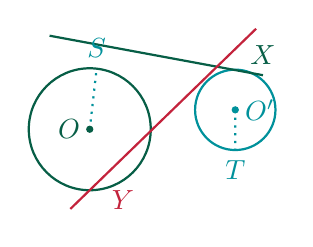
\begin{tikzpicture}[scale=0.88]
    \draw[thick, color=brandNavy] (0,0) circle (0.88);
    \draw[thick, color=brandBlue] (2.1,0.28) circle (0.58);
    \coordinate (O) at (0,0);
    \coordinate (O1) at (2.1,0.28);
    \coordinate (X) at (1.9, 1.05);
    \coordinate (Y) at (0.48, -0.75);
    \draw[thick, color=brandNavy] (-0.58, 1.35) -- (2.5, 0.78) node[above] {$X$};
    \draw[thick, color=brandCrimson] (-0.28, -1.15) -- (2.4, 1.45);
    \draw[thick, dotted, color=brandBlue] (O) -- (0.1, 0.88) node[above] {$S$};
    \draw[thick, dotted, color=brandBlue] (O1) -- (2.1, -0.3) node[below] {$T$};
    \node[below, color=brandCrimson] at (Y) {$Y$};
    \fill[brandNavy] (O) circle (1.5pt) node[left] {$O$};
    \fill[brandBlue] (O1) circle (1.5pt) node[right] {$O'$};
  \end{tikzpicture}
\end{minipage}
\end{khcard}

\vspace{4pt}
\begin{khcard}
\begin{minipage}[c]{0.65\textwidth}
  \exhead{២} គេមាន $MA, MB$ និង $MC$ ជាបន្ទាត់ប៉ះ\\
  ទៅនឹងរង្វង់ផ្ចិត $O$ និងផ្ចិត $O'$ ។ ចូរបង្ហាញថា $MA = MC$ ។
\end{minipage}\hfill
\begin{minipage}[c]{0.33\textwidth}
  \centering
  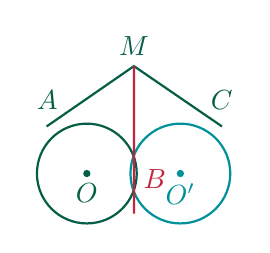
\begin{tikzpicture}[scale=0.88]
    \draw[thick, color=brandNavy] (0,0) circle (0.72);
    \draw[thick, color=brandBlue] (1.35,0) circle (0.72);
    \coordinate (O) at (0,0);
    \coordinate (O1) at (1.35,0);
    \coordinate (M) at (0.68, 1.55);
    \draw[thick, color=brandNavy] (-0.58, 0.68) -- (M) node[above] {$M$} -- (1.95, 0.68);
    \draw[thick, color=brandCrimson] (M) -- (0.68, -0.58);
    \node[above left, color=brandNavy] at (-0.28, 0.78) {$A$};
    \node[above right, color=brandNavy] at (1.65, 0.78) {$C$};
    \node[below right, color=brandCrimson] at (0.68, 0.2) {$B$};
    \fill[brandNavy] (O) circle (1.5pt) node[below] {$O$};
    \fill[brandBlue] (O1) circle (1.5pt) node[below] {$O'$};
  \end{tikzpicture}
\end{minipage}
\end{khcard}

\vspace{4pt}
\begin{khboxpractice}
  \phead\ គេមានរង្វង់ពីរមានទំហំខុសគ្នាដែលមានផ្ចិត $O$ និង $O'$ ។ រង្វង់ទាំងពីរនេះមានបន្ទាត់ប៉ះរួមមួយ ដែលមានចម្ងាយរវាងផ្ចិតទាំងពីរស្មើនឹង $4\text{cm}$ និងមានចម្ងាយរវាងផ្ចិត $1\text{cm}$ ដូចរូបខាងក្រោម ។ ចូរគណនាកាំនៃរង្វង់ទាំងពីរ ។

\vspace{3pt}
\begin{center}
  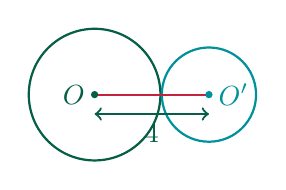
\begin{tikzpicture}[scale=0.88]
    \draw[thick, color=brandNavy] (0,0) circle (0.95);
    \draw[thick, color=brandBlue] (1.65,0) circle (0.68);
    \coordinate (O) at (0,0);
    \coordinate (O1) at (1.65,0);
    \draw[thick, color=brandCrimson] (O) -- (O1);
    \draw[<->, thick, color=brandNavy] (0,-0.28) -- (1.65,-0.28) node[midway, below] {$4$};
    \fill[brandNavy] (O) circle (1.5pt) node[left] {$O$};
    \fill[brandBlue] (O1) circle (1.5pt) node[right] {$O'$};
  \end{tikzpicture}
  \hspace{1.5cm}
  \begin{tikzpicture}[scale=0.88]
    \draw[thick, color=brandNavy] (0,0) circle (0.95);
    \draw[thick, color=brandBlue] (0.38,0) circle (0.58);
    \coordinate (O) at (0,0);
    \coordinate (O1) at (0.38,0);
    \draw[thick, color=brandNavy] (O) -- (0.38,0);
    \draw[<->, thick, color=brandCrimson] (0,0.18) -- (0.38,0.18) node[midway, above] {$1$};
    \fill[brandNavy] (O) circle (1.5pt) node[below] {$O$};
    \fill[brandBlue] (O1) circle (1.5pt) node[below] {$O'$};
  \end{tikzpicture}
\end{center}
\end{khboxpractice}

\vspace{10pt}
\begin{center}
  \begin{tikzpicture}
    \node[anchor=west] at (0,0) {\fontsize{11}{11}\selectfont\kml\color{brandCrimson}\ding{45} \textbf{ខំរកទើបមាន ខំរៀនទើបចេះ}};
    \draw[line width=1.5pt, color=brandNavy] (6.8, 0) -- (13.5, 0);
    \node[anchor=west] at (13.7,0) {\color{brandGold}\Large $\spadesuit\spadesuit$};
  \end{tikzpicture}
\end{center}

\end{document}
